\documentclass[conference]{IEEEtran}


\usepackage{macro}

\IEEEoverridecommandlockouts
% The preceding line is only needed to identify funding in the first footnote. If that is unneeded, please comment it out.
\usepackage{cite}
\usepackage{amsmath,amssymb,amsfonts}
\usepackage{algorithm}
\usepackage{graphicx}
\usepackage{textcomp}
\usepackage{xcolor}

\def\BibTeX{{\rm B\kern-.05em{\sc i\kern-.025em b}\kern-.08em
    T\kern-.1667em\lower.7ex\hbox{E}\kern-.125emX}}
\begin{document}

\title{Safe and Near Optimal Controller Synthesis for Stochastic Hybrid Systems\\
{\footnotesize \textsuperscript{*}N....}
\thanks{Identify applicable funding agency here. If none, delete this.}
}

\author{\IEEEauthorblockN{1\textsuperscript{st} Richard Valentin Yantas Alcantara}
\IEEEauthorblockA{\textit{dept. name of organization (of Aff.)} \\
\textit{name of organization (of Aff.)}\\
Arequipa, Peru \\
email address}
\and
\IEEEauthorblockN{2\textsuperscript{nd} Marco Muniz}
\IEEEauthorblockA{\textit{dept. name of organization (of Aff.)} \\
\textit{name of organization (of Aff.)}\\
City, Country \\
email address}

}

\maketitle


\maketitle

\begin{abstract}
    Stochastic hybrid systems allow to model the interaction between continuos dynamics,
discrete dynamics and probabilistic uncertainty. Because of their versatility,
stochastic hybrid systems have emerged as a powerful framework for capturing 
the intricacies of complex systems. Motivated by this, considerable research effort 
has been devoted to the development of modeling analysis and control 
methods for stochastic hybrid systems. 
% Goals, results.

\end{abstract}

\begin{IEEEkeywords}
SHG, formatting, style, styling, insert
\end{IEEEkeywords}

\section{Introduction}
Hybrid systems are widely used in engineering applications and its 
importance has grown up considerably these last years, because of their 
ease of implementation for controlling cyber-physical systems.
A switched systems is a set of dynamical systems, each with its own 
dynamical behaviour controlled by a parameter mode $u$ whose values 
are in a finite set. However, due to the composition of many switched 
systems together, the global switched systems has a number of modes 
and dynamics which increases exponentially. Switched systems have 
numerous applications in control of mechanical systems, the automotive
 industry, and many other fields.


\section{Preliminaries}

In this section we summaries the basic definition of stochastic hybrid games, 
their concrete and symbolic semantics and the safety system implemented 
underlying the currently distributed version of UPPAAL.\cite{larsen2016online}


\subsection{Sthocastic Hybrid Game}

\textbf{Definitiom 1}\emph{(Stochastic Hybrid Game)}. A stochastic hybrid
game $\mathcal{G}_{n,m} = (\mathcal{C,U,X,F},\delta)$ where:



\begin{itemize}
    \item \emph{$\mathcal{C}$ is a controller with a finite set of(controllable) modes C }.
    \item \emph{$\mathcal{U}$ is a controller with a finite set of(uncontrollable) modes U }.
    \item \emph{$X = \left\{ x_{1},...,x_{n}  \right\}$ is a finite set of continuos (real-valued) varibales,}.
    \item \emph{ for each c $\in$ C and u $\in$ U,  $\mathcal{F}_{c,u} : \mathbb{R}_{>0} \times
     \mathbb{R}^{X} \rightarrow  \mathbb{R}^{X}$ is the flow-function that describe the 
     evolution of the continuos variables over time in the combined mode (c,u), and  }
    \item \emph{ $\delta$ is a family of density functions, $\delta_\gamma(\tau,u') $ is the
    density that $\mathcal{U}$ in the global configuration $\gamma = (c,u,v)$ will change to 
    the uncontrollable mode $u'$ after a delay of $\tau^{4}$.  }
    
\end{itemize}







\subsection{Sthocastic Hybrid Systems Safety Definitions}



In this part is presented a method based on correction by design of
 discrete linear switched system in the time. the method consist of 
 given a objective region \emph{R} of state space, the method built 
 a set \emph{S} and a control that guide any element from  \emph{S} 
 a \emph{R}. This method works in an iterative way to back to reach 
 the region \emph{R}. The method  can also be used for synthesize 
 a stability control that is keep inside of R, whole states start in
  \emph{R}.

In order to find safety pattern to our system we  use a
decomposition algorithm, which explore in a binary way regions which
guarantee a beviouring inside to restrictions. \cite{le2017improved}

  \textbf{Problem 1}\emph{(Control Synthesis Problem)}. Let us 
consider a sampled Hybrid System. Given three sets R,S and B, 
with ${R \cup B \in S}$  and ${R \cap B = \varnothing }$ find a 
rule ${\sigma(.)}$ such that, for any ${x(0) \in R }$. 

\begin{itemize}
    \item \emph{ ${\tau}$-stability: ${x(t)}$ return in R 
    infinitely often, at some multiples of sampling time ${\tau}$}.
    \item \emph{ safety: ${x(t)}$ always stays in ${S/B}$.}
\end{itemize}




 \textbf{Problem 2} \emph{((R,S) - Stability Problem)}. Given a 
 switched system, a set of recurrence 
 ${\mathbb{R}^n}$ and a safe set \emph{S} ${\subset \mathbb{R}^n}$,find a control rule 
 ${\sigma : \mathbb{R}^+ \rightarrow U}$ such that, for any
  initial condition ${x_0  \in  R_1}$ and any perturbation 
  ${\varpi :\mathbb{R}^+\rightarrow U}$  the
   following holds:
 
 \begin{itemize}
    \item \emph{ Recurrence in \emph{R}:there are a monotonically 
    strictly increasing sequence of (positive) integers
    ${k_t, t \in \mathbb{N}}$ such that for all ${ t \in \mathbb{R}^n,
    \phi(k_l\tau;t_0,x^0,\sigma,w) \in \mathbb{R} }$.}

    \item \emph{ Stability in \emph{S}: for all ${ t \in \mathbb{R}^n,
    \phi(t;t_0,x^0,\sigma,w) \in S}$ .}
\end{itemize}


 
\textbf{Problem 3} \emph{((${R_1,R_2,S}$) - Reachability problem).
Given a switched system of the form shown above, two sets  
${ R_1 \subset \mathbb{R}^n}$  and ${ R_2 \subset \mathbb{R}^n}$ 
and a safety set  ${S \subset  \mathbb{R}^n}$, find a control rule 
${\sigma}$ :
${\mathbb{R}^+\rightarrow U}$ such that, for any initial condition 
${x_0  \in  R_1}$ and any perturbation  ${\varpi : \mathbb{R}^+  
\rightarrow U}$, the following holds:}

\begin{itemize}
  \item  \emph{Reachability from ${R_1}$ to ${R_2}$: there exists 
  an integer ${k \in \mathbb{N} }$ such that we have ${ \phi( k_l\tau
  ;t_0,x^0,\sigma,w) \in R_2 }$.}
  
  \item \emph{ Stability in S: for all ${ t \in \mathbb{R}^+, 
  \phi(t;t_0,x^0,\sigma,w) \in S}$ .}
\end{itemize}


\section{Case Study: Solar Water Heating}


\subsection{Solar Water Heating as Sthocastic Hybrid Game}

The hybrid solar water heating scenario with 12 modes of operations is
defined  like this: $\mathcal{G}_{n,m} = (\mathcal{C,U,X,F},\delta)$, 
where the controller $\mathcal{C}$ has a finite set of controllable modes,
given by resistance state ${r \in \mathbb{B} = \left\lbrace 0,1 \right\rbrace }$ 
and piston movement $p \in \left\lbrace-1,0,1\right\rbrace $. 
The environment $\mathcal{U}$ has a finite set of uncontrollable modes
 $v \in \mathbb{B} $, that means the valve state for opening/closing
water aperture. We assume that $\mathcal{U}$ given $\delta$ can switch
among modes with equal probability at every period $\tau$. The state variables
in $\mathcal{X}_{(t)}$ are given by $\left\lbrace \tcont,\vcont,\energy \right\rbrace $, 
tank temperature, tank volumen and energy consumption respectively. Also 
Disturbance effect is considered in the dynamical system such as environment
temperature, water input temperature and irradiance as a uncontrollable 
continuos environment variables.


\begin{align}
    \frac{d}{dt}\tcont &=   -\frac{1}{\vcont}  \constone(\tcont-\tenv) - 
    \frac{ \textbf{v} }{\vcont}\consttwo (\tcont-\tin) + \notag\\ &\qquad +
    \textbf{r} \frac{ \constthree \auxheat  }{\vcont}  + 
    \frac{ \constfour \irradiance}{\vcont} 
\label{temperature-equation}
\end{align}

\begin{equation}
    \frac{d}{dt}\vcont = -k \textbf{p}; \quad
% \frac{d}{dt}\vcont = k .sgn(100 \textbf{p}  - \vcont); \quad
\label{volume-equation}
\end{equation}

\begin{equation} 
\frac{d}{dt}\energy =  \textbf{r}  \auxheat ;
\label{Energy-equation}
\end{equation}

In equation \ref{temperature-equation}. the paremeters,  $\left\lbrace 
\constone, \consttwo, \constthree, \constfour \right\rbrace $ 
remains constant in time. In equation \ref{volume-equation}, 
\emph{k} is the piston velocity.


\subsection{Discrete Model}

We use uppaal stratego to model our system:

\begin{figure}[h]  % \begin{figure}[h]
  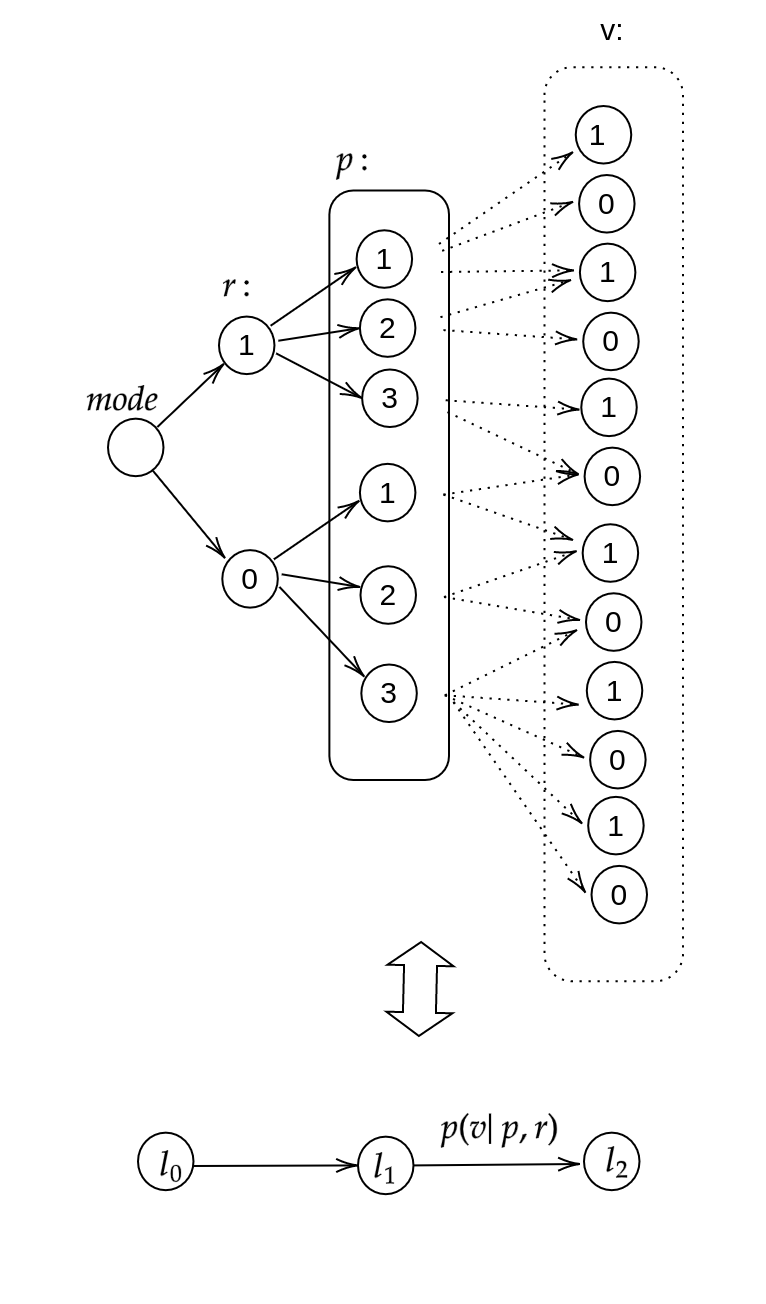
\includegraphics[scale = 0.25]{4}
  \caption{Explotion Transition system}
  \centering
\end{figure}


\section{Experiments}

\subsection{Enviornment data}
In our system we can notice some variables wich are influenced by the enviorment,
in order to be more realistic, we have used data from the spain sity named sevilla.
Data such as temperature and irradiance is got during 1 year which a timestep 
of 15 minutes.

\begin{figure}[H]  % \begin{figure}[h]
  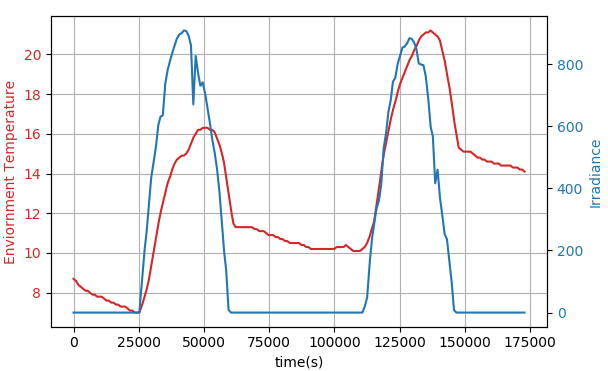
\includegraphics[scale = 0.35]{7}
  \caption{Controllable and uncontrollable variables signals}
  \centering
\end{figure}



\subsection{Solar Water Heating simulation}\label{AA}

The is managed by discrete controllable and uncontrollable variables 
which are defined by our controller and probabilities events.

\begin{figure}[H]  % \begin{figure}[h]
  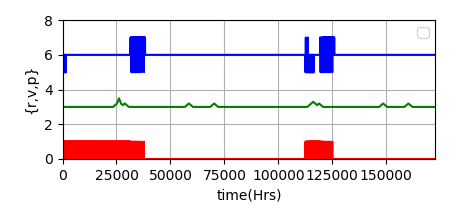
\includegraphics[scale = 0.5]{3_1}
  \caption{Controllable and uncontrollable variables signals}
  \centering
\end{figure}


  

Considering the disturbance,controllable modes and uncontrollable modes we get 
asd a result:

\begin{figure}[H]  % \begin{figure}[h]
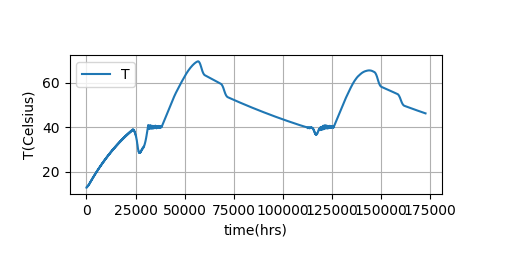
\includegraphics[scale = 0.5]{1}
\caption{Container tempeature state in time}
\centering
\end{figure}



Each controller has its performance, a simple controller is implemented as
a reference to our controller synthesis. As it is  shown we can notice what 
kind of performance is provided over our case of study.

\begin{figure}[H]
  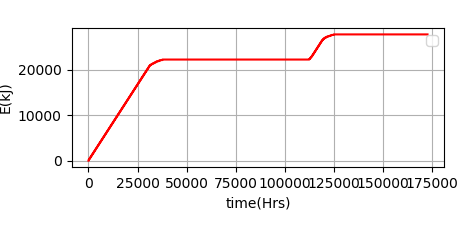
\includegraphics[scale = 0.5]{3_2}
  \caption{ Energy consumption in time}
  \centering
\end{figure}


As decribed we need to guarantee a safety system in that sense we import some 
functionalities through Ibex C++ it imples to work with intervals in order
to find a safety patterns. In this case it is basically restricted by simple
constraints.

\begin{figure}[H]  % \begin{figure}[h]
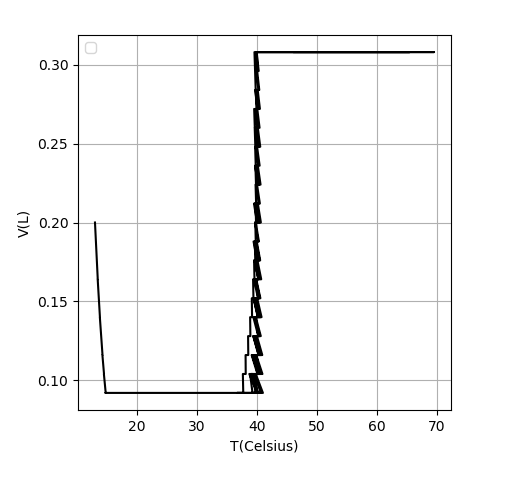
\includegraphics[scale = 0.4]{5}
\centering
\caption{Safety state space temperature-Volumen}
\centering
\end{figure}
  




\subsection{Strategy Controller Synthesis}
\begin{itemize}
\item  ...
\end{itemize}




\subsection{Figures and Tables}
\paragraph{Positioning Figures and Tables} Place figures and tables at the top and 


\begin{table}[htbp]
\caption{Table Type Styles}
\begin{center}
\begin{tabular}{|c|c|c|c|}
\hline
\textbf{Table}&\multicolumn{3}{|c|}{\textbf{Table Column Head}} \\
\cline{2-4} 
\textbf{Head} & \textbf{\textit{Table column subhead}}& \textbf{\textit{Subhead}}& \textbf{\textit{Subhead}} \\
\hline
copy& More table copy$^{\mathrm{a}}$& &  \\
\hline
\multicolumn{4}{l}{$^{\mathrm{a}}$Sample of a Table footnote.}
\end{tabular}
\label{tab1}
\end{center}
\end{table}

%\begin{figure}[htbp]
%\centerline{
\includegraphics{fig1.png}}
%\caption{Example of a figure caption.}
%\label{fig}
%\end{figure}






\section{Conclusions and Future work}


\section{References}

\bibliographystyle{plain}  %Internal Style
\bibliography{mybib}
\end{document}
%\addcontentsline{toc}{chapter}{Bibliography}
